%------------------------------------------------------------------------------
\chapter{Appendix}
\label{sec:app}
%------------------------------------------------------------------------------

\section*{Number of Events and Event Yield}

\begin{table}[H]
\centering
\begin{tabular}{|r|r|r|r|r|}
\toprule
Datasets & $N$ PS & $N$ SR & Yield PS & Yield SR \\
\midrule
\midrule
$t\bar{t}t\bar{t}$ NLO & 444664 & 301420 & 47.74 & 29.75 \\
$t\bar{t}t\bar{t}$ LO & 452548 & 283457 & 34.36 & 21.15 \\
$t\bar{t}W$ & 391298 & 14170 & 973.75 & 61.37 \\
$t\bar{t}WW$ & 4370 & 876 & 38.44 & 7.51 \\
$t\bar{t}Z$ & 539828 & 63621 & 630.52 & 50.06 \\
$t\bar{t}H$ & 439753 & 41043 & 324.39 & 38.95 \\
$t\bar{t}$QmisID & 11359 & 586 & 1039.16 & 13.63 \\
$t\bar{t}$CO & 5993 & 759 & 515.92 & 21.84 \\
$t\bar{t}$HF & 17144 & 462 & 1881.69 & 15.89 \\
$t\bar{t}$light & 2100 & 292 & 128.40 & 6.72 \\
$t\bar{t}$others & 1977 & 195 & 153.27 & 6.28 \\
$t(\bar{t})X$ & 26538 & 926 & 198.14 & 5.12 \\
$VV$ & 275409 & 1890 & 313.04 & 4.39 \\
$V$+jets & 6284 & 81 & 841.23 & 1.63 \\
others & 2579 & 8453 & 42.33 & 3.06 \\
\bottomrule
\end{tabular}
\caption{Number of simulated data events $N$ and Yields after applying the Pre-Section PS and inside the Signal Region SR.}
\label{tab:prevssr}
\end{table}

\section*{Input Features}
\label{ap:Input}

\subsection*{Feedforward Neural Network}

\begin{figure}[H]
\begin{subfigure}{.5\textwidth}
  \centering
  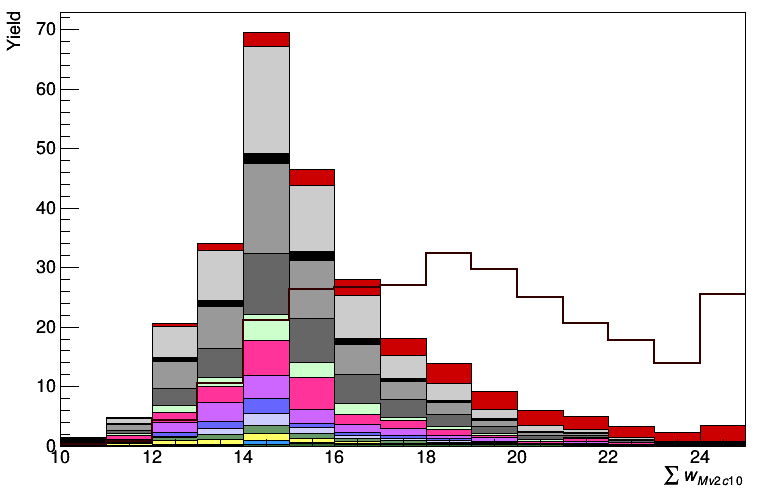
\includegraphics[width=.99\linewidth]{figs/features/MV2c10}
\end{subfigure}%
\begin{subfigure}{.5\textwidth}
  \centering
  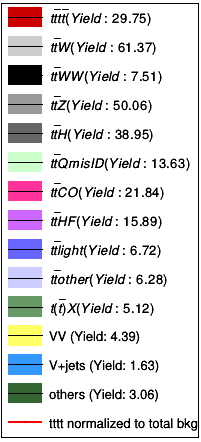
\includegraphics[width=.29\linewidth]{figs/features/legende}
\end{subfigure}
\begin{subfigure}{.5\textwidth}
  \centering
  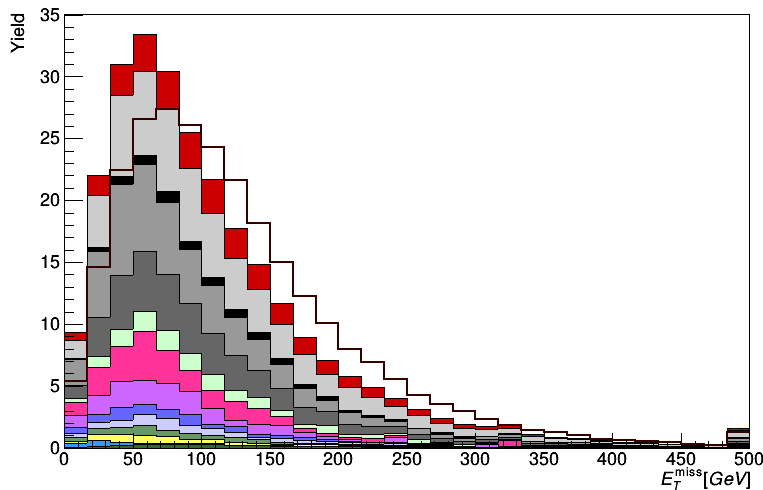
\includegraphics[width=.99\linewidth]{figs/features/met_met}
\end{subfigure}%
\begin{subfigure}{.5\textwidth}
  \centering
  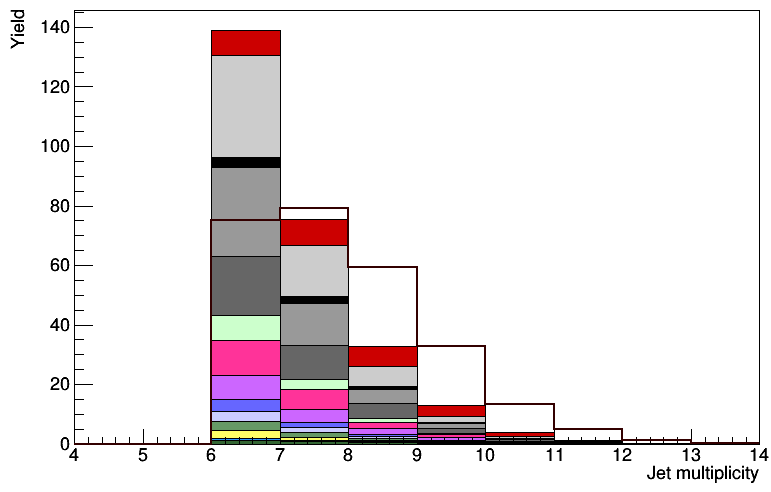
\includegraphics[width=.99\linewidth]{figs/features/nJets}
\end{subfigure}
\begin{subfigure}{.5\textwidth}
  \centering
  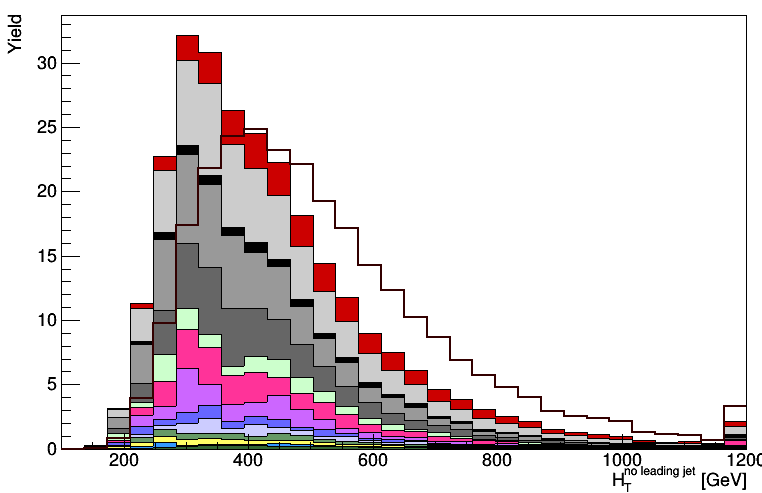
\includegraphics[width=.99\linewidth]{figs/features/HT_jets_noleadjet}
\end{subfigure}
\begin{subfigure}{.5\textwidth}
  \centering
  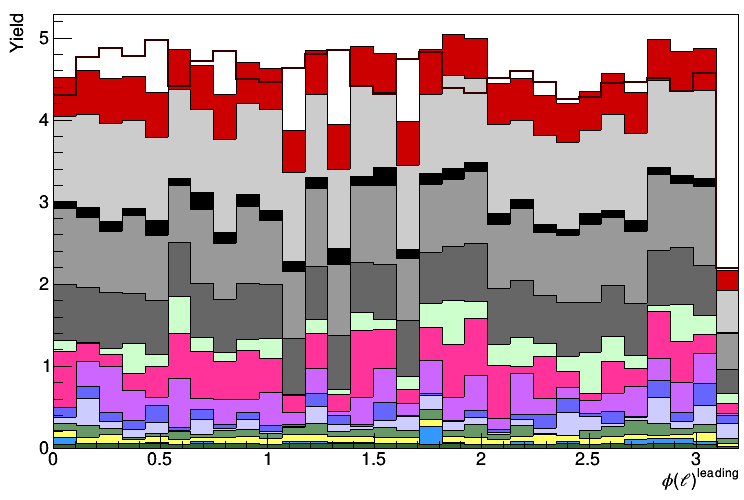
\includegraphics[width=.99\linewidth]{figs/features/lep_0_phi}
\end{subfigure}%
\caption{Input features of the Feedforward Neural Network.}
\end{figure}

\newpage

\begin{figure}[H]
\begin{subfigure}{.5\textwidth}
  \centering
  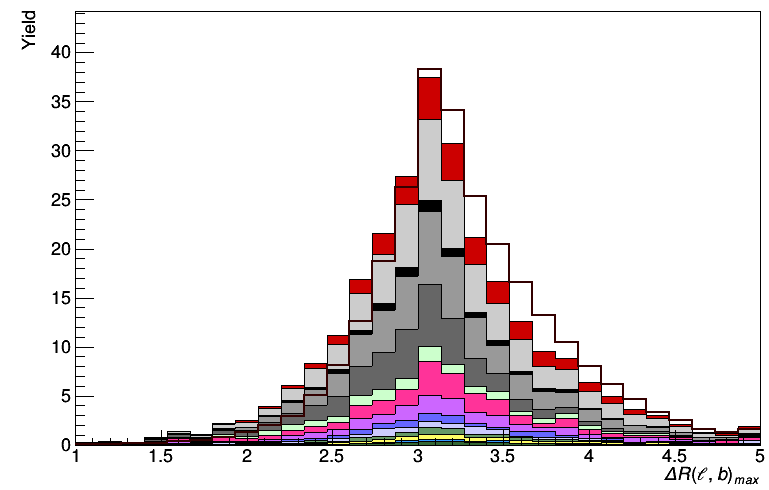
\includegraphics[width=.99\linewidth]{figs/features/deltaR_lb_max}
\end{subfigure}%
\begin{subfigure}{.5\textwidth}
  \centering
  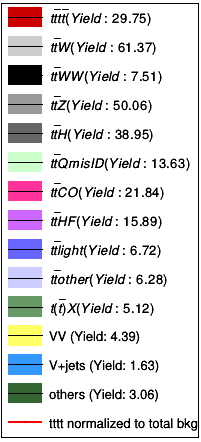
\includegraphics[width=.29\linewidth]{figs/features/legende}
\end{subfigure}
\begin{subfigure}{.5\textwidth}
  \centering
  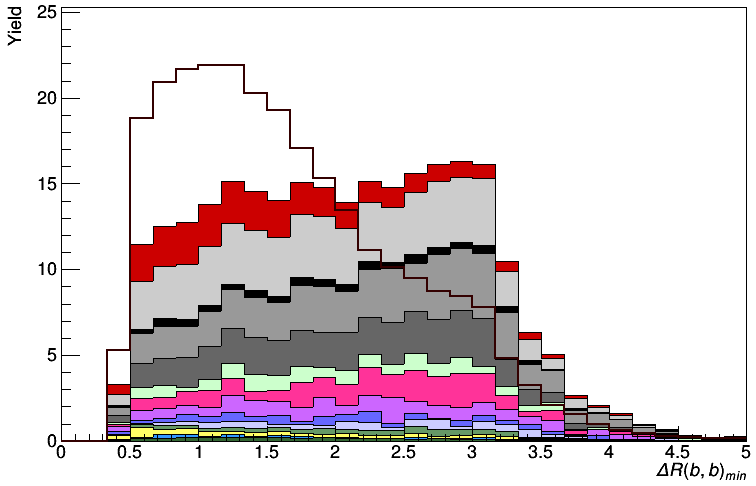
\includegraphics[width=.99\linewidth]{figs/features/dRbbmin}
\end{subfigure}%
\begin{subfigure}{.5\textwidth}
  \centering
  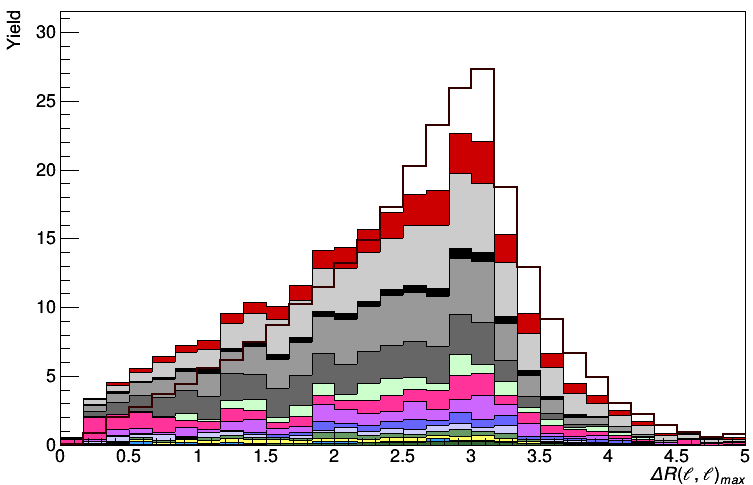
\includegraphics[width=.99\linewidth]{figs/features/deltaR_ll_max}
\end{subfigure}
\begin{subfigure}{.5\textwidth}
  \centering
  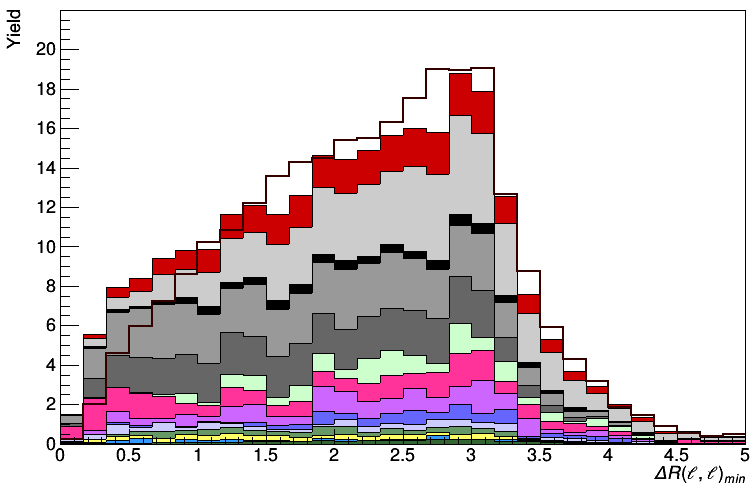
\includegraphics[width=.99\linewidth]{figs/features/deltaR_ll_min}
\end{subfigure}
\begin{subfigure}{.5\textwidth}
  \centering
  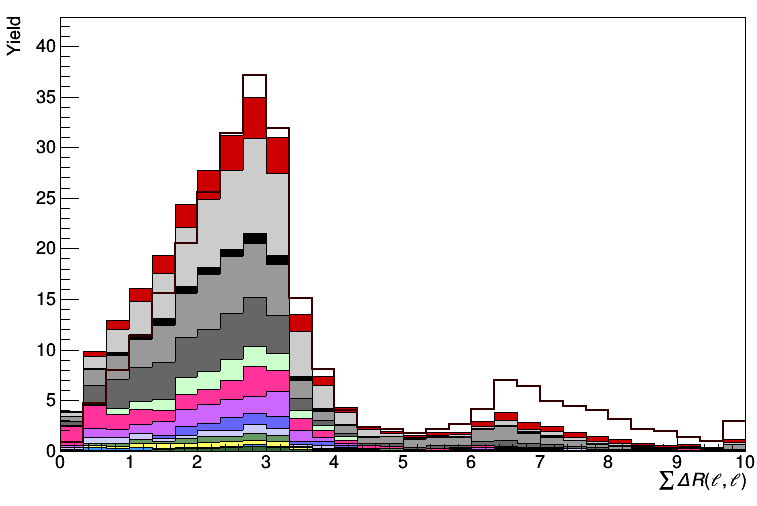
\includegraphics[width=.99\linewidth]{figs/features/deltaR_ll_sum}
\end{subfigure}
\begin{subfigure}{.5\textwidth}
  \centering
  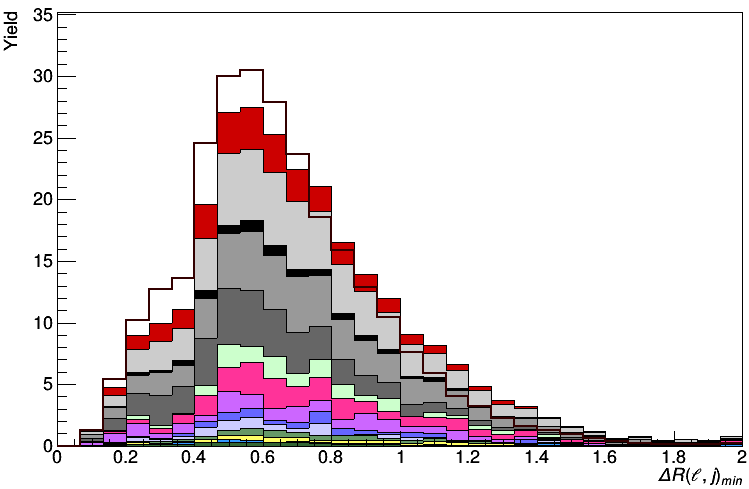
\includegraphics[width=.99\linewidth]{figs/features/deltaR_lj_min}
\end{subfigure}%
\begin{subfigure}{.5\textwidth}
  \centering
  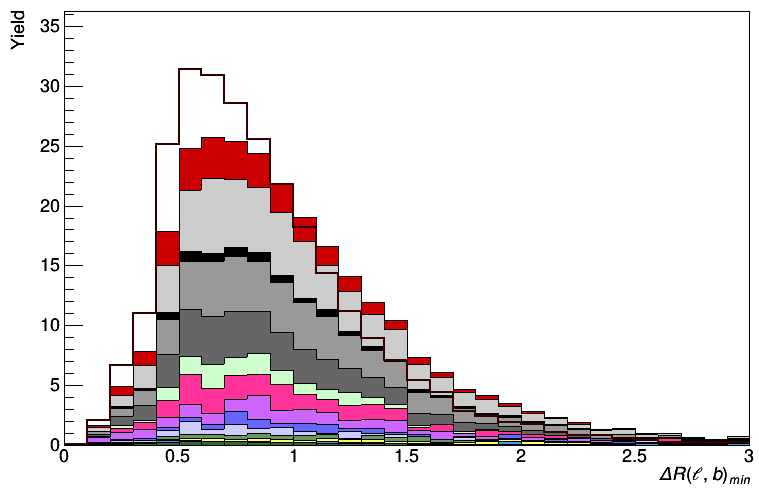
\includegraphics[width=.99\linewidth]{figs/features/deltaR_lb_min}
\end{subfigure}
\caption{$\Delta R$ input features of the Feedforward Neural Network.}
\end{figure}

\newpage


\begin{figure}[H]
\begin{subfigure}{.5\textwidth}
  \centering
  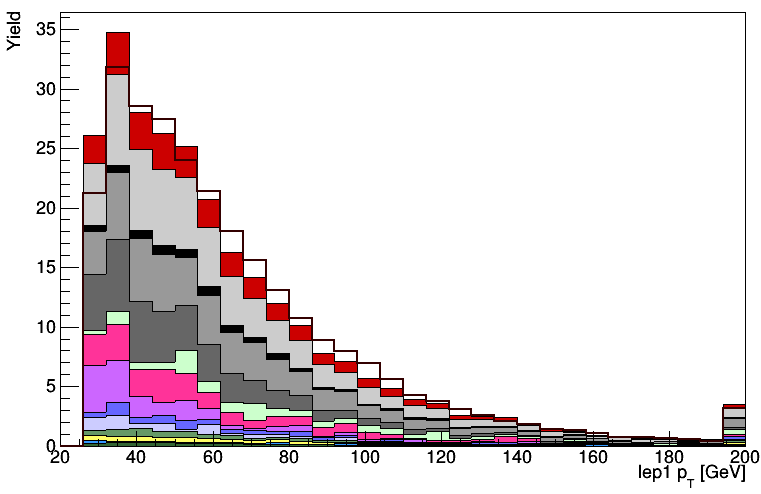
\includegraphics[width=.99\linewidth]{figs/features/lep_1_pt}
\end{subfigure}%
\begin{subfigure}{.5\textwidth}
  \centering
  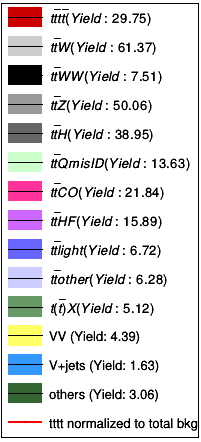
\includegraphics[width=.29\linewidth]{figs/features/legende}
\end{subfigure}
\begin{subfigure}{.5\textwidth}
  \centering
  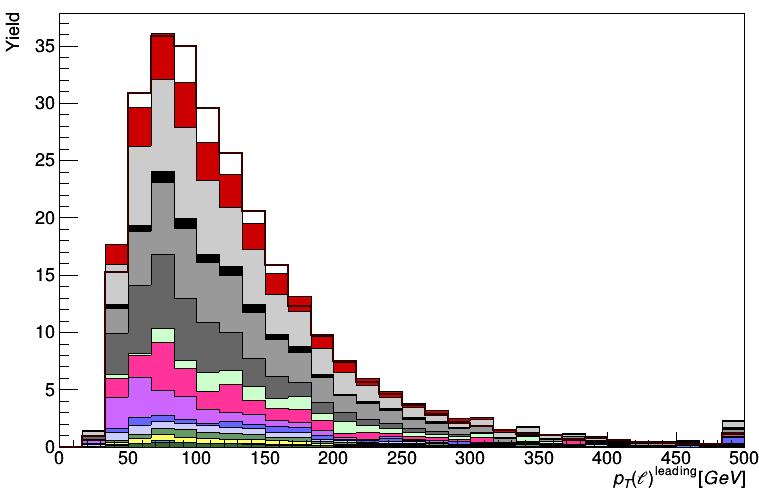
\includegraphics[width=.99\linewidth]{figs/features/lep_0_pt}
\end{subfigure}%
\begin{subfigure}{.5\textwidth}
  \centering
  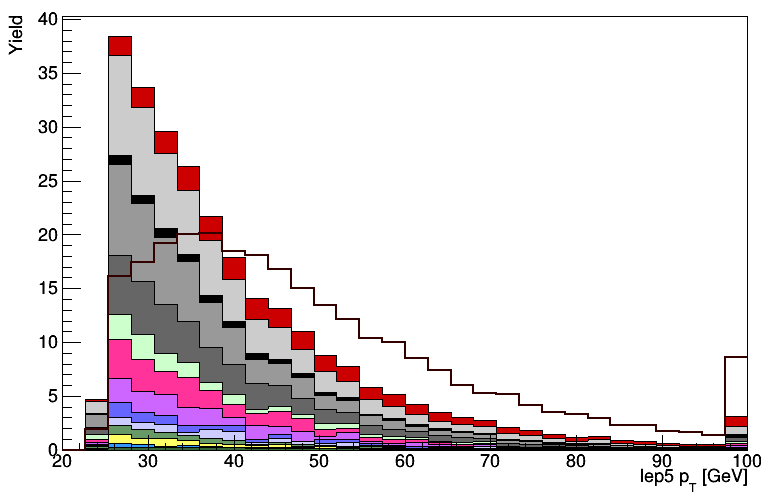
\includegraphics[width=.99\linewidth]{figs/features/jet_5_pt}
\end{subfigure}
\begin{subfigure}{.5\textwidth}
  \centering
  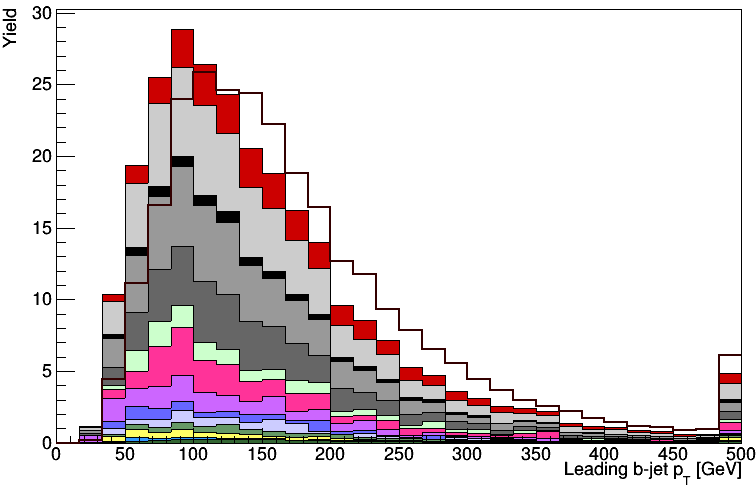
\includegraphics[width=.99\linewidth]{figs/features/leading_bjet_pT}
\end{subfigure}
\begin{subfigure}{.5\textwidth}
  \centering
  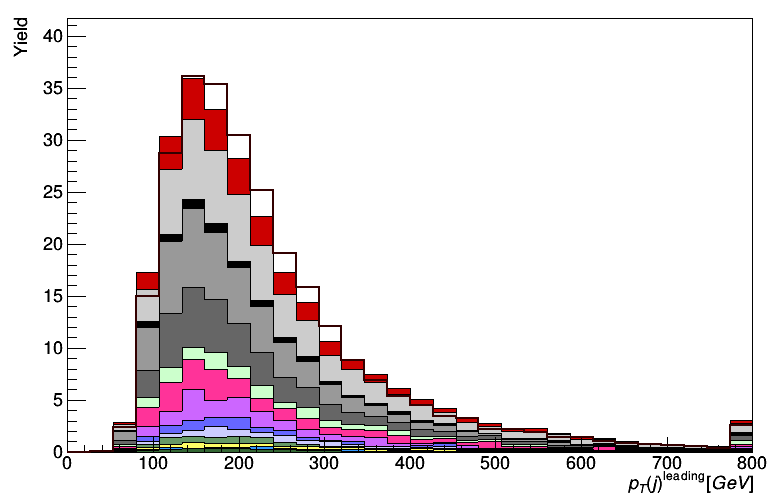
\includegraphics[width=.99\linewidth]{figs/features/leading_jet_pT}
\end{subfigure}
\begin{subfigure}{.5\textwidth}
  \centering
  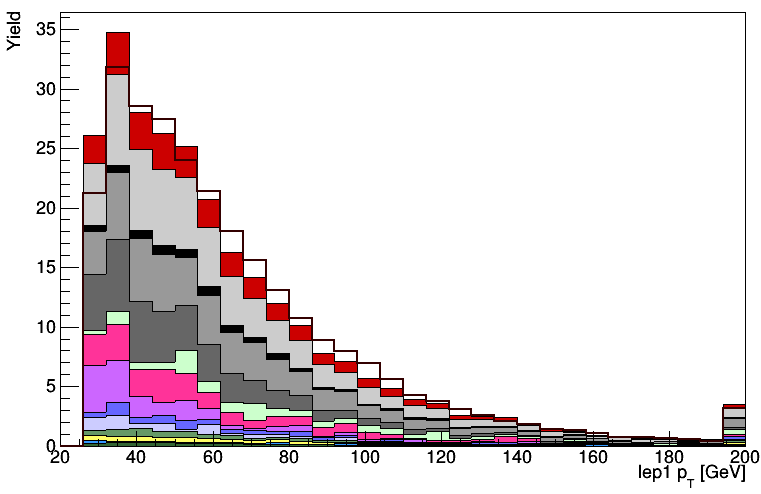
\includegraphics[width=.99\linewidth]{figs/features/lep_1_pt}
\end{subfigure}
\caption{$p_{\text{T}}$ input features of the Feedforward Neural Network.}
\end{figure}

\newpage

\subsection*{Recurrent Neural Network}

The distributions show in this sub-section are the input Features of the RNN to gather $\sum w_{\text{MV2c10}}$, $E_{T}^{miss}$ and $N_j$. The yield of the features varies depending on the particle type

\begin{figure}[H]
\begin{subfigure}{.5\textwidth}
  \centering
  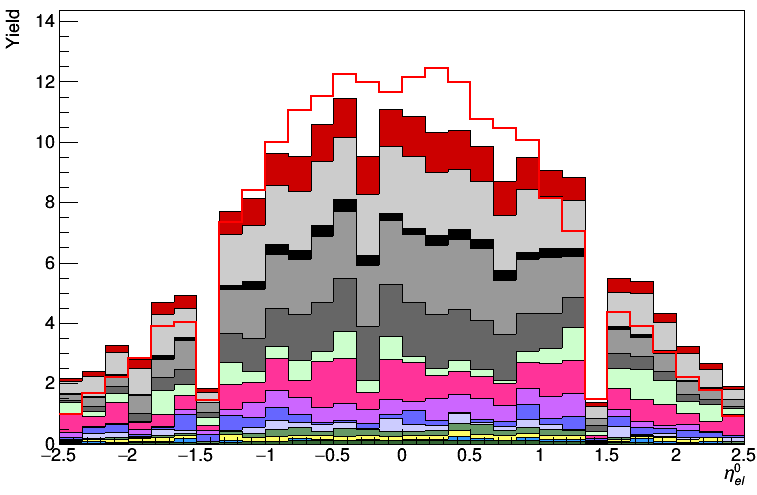
\includegraphics[width=.99\linewidth]{figs/featuresRNN/el_eta_0}
\end{subfigure}%
\begin{subfigure}{.5\textwidth}
  \centering
  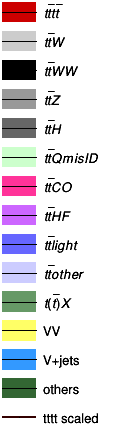
\includegraphics[width=.29\linewidth]{figs/featuresRNN/Legend_wo}
\end{subfigure}
\begin{subfigure}{.5\textwidth}
  \centering
  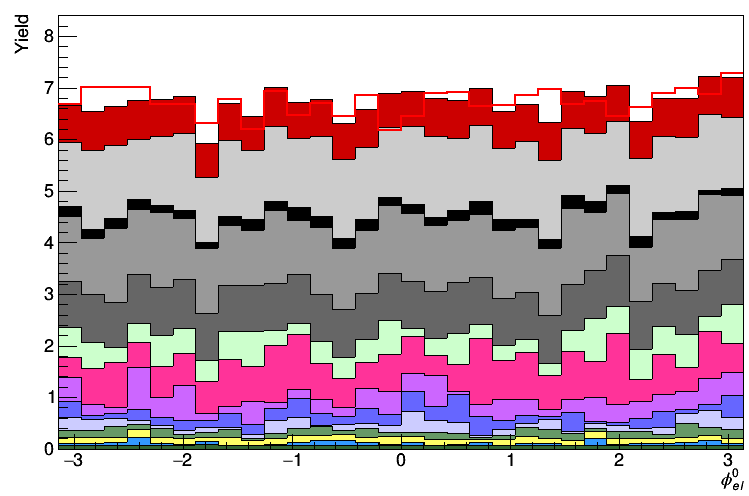
\includegraphics[width=.99\linewidth]{figs/featuresRNN/el_phi_0}
\end{subfigure}%
\begin{subfigure}{.5\textwidth}
  \centering
  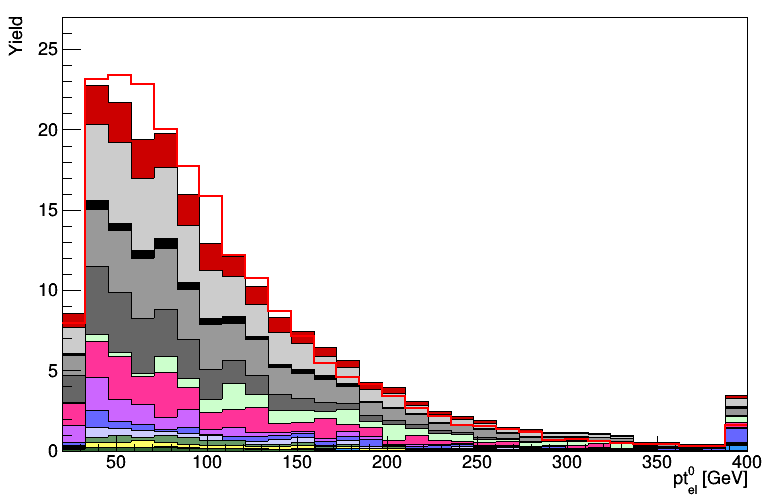
\includegraphics[width=.99\linewidth]{figs/featuresRNN/el_pt_0}
\end{subfigure}
\begin{subfigure}{.5\textwidth}
  \centering
  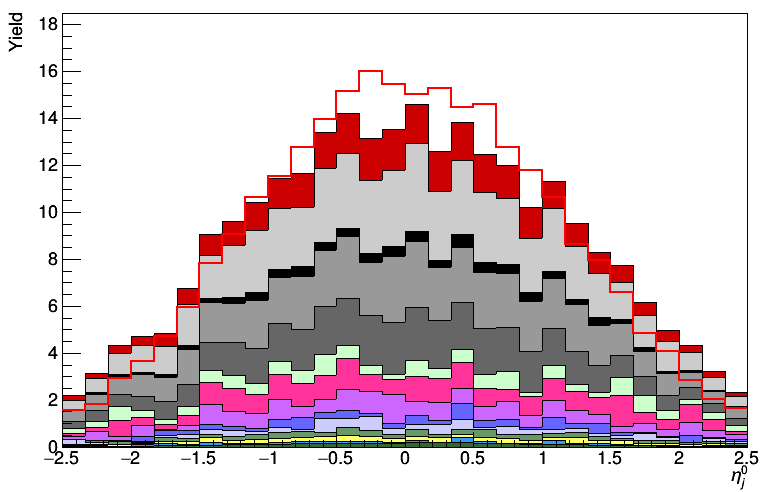
\includegraphics[width=.99\linewidth]{figs/featuresRNN/jet_eta_0}
\end{subfigure}
\caption{Input features of the Recurrent Neural Network.}
\end{figure}


\begin{figure}[H]
\begin{subfigure}{.5\textwidth}
  \centering
  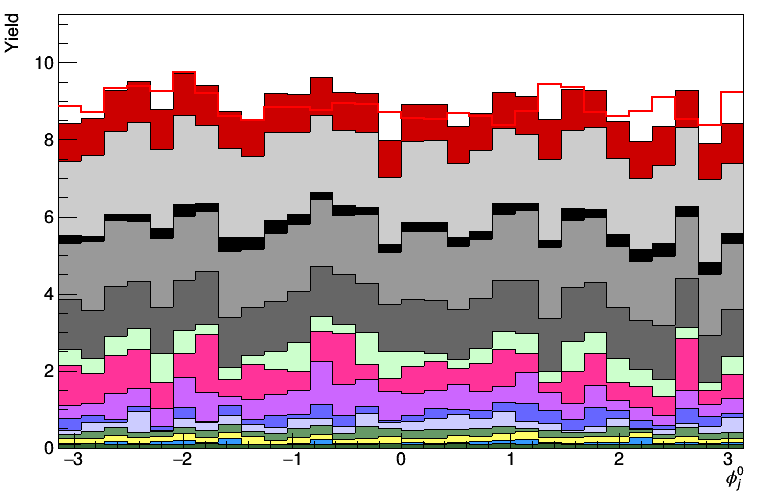
\includegraphics[width=.99\linewidth]{figs/featuresRNN/jet_phi_0}
\end{subfigure}
\begin{subfigure}{.5\textwidth}
  \centering
  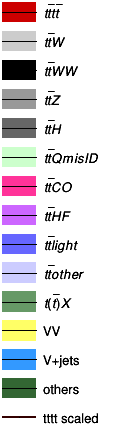
\includegraphics[width=.29\linewidth]{figs/featuresRNN/Legend_wo}
\end{subfigure}
\begin{subfigure}{.5\textwidth}
  \centering
  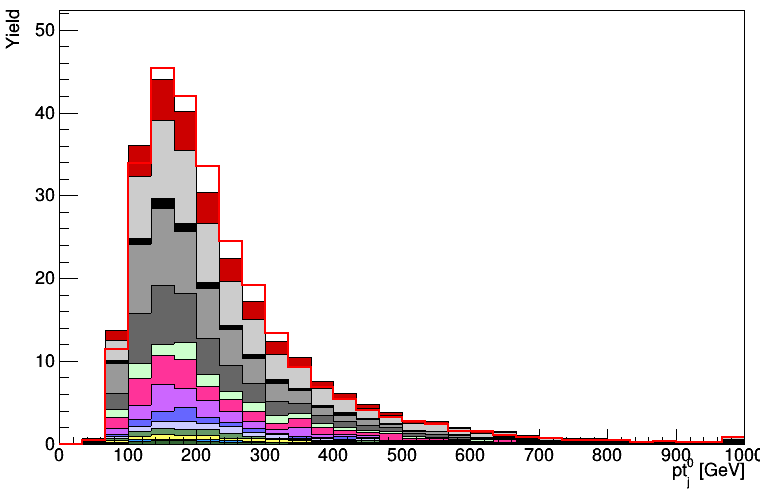
\includegraphics[width=.99\linewidth]{figs/featuresRNN/jet_pt_0}
\end{subfigure}%
\begin{subfigure}{.5\textwidth}
  \centering
  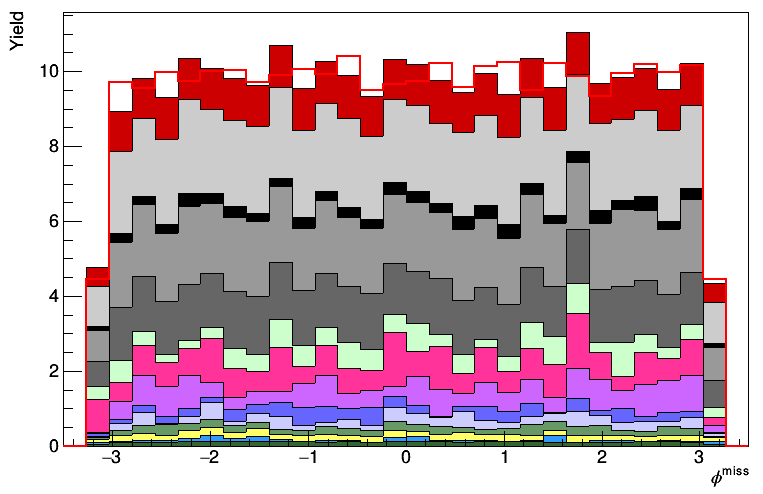
\includegraphics[width=.99\linewidth]{figs/featuresRNN/met_phi}
\end{subfigure}
\begin{subfigure}{.5\textwidth}
  \centering
  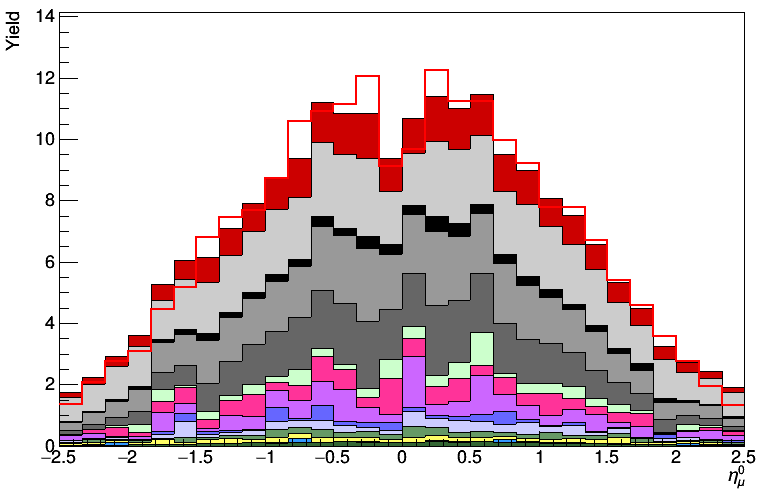
\includegraphics[width=.99\linewidth]{figs/featuresRNN/mu_eta_0}
\end{subfigure}
\begin{subfigure}{.5\textwidth}
  \centering
  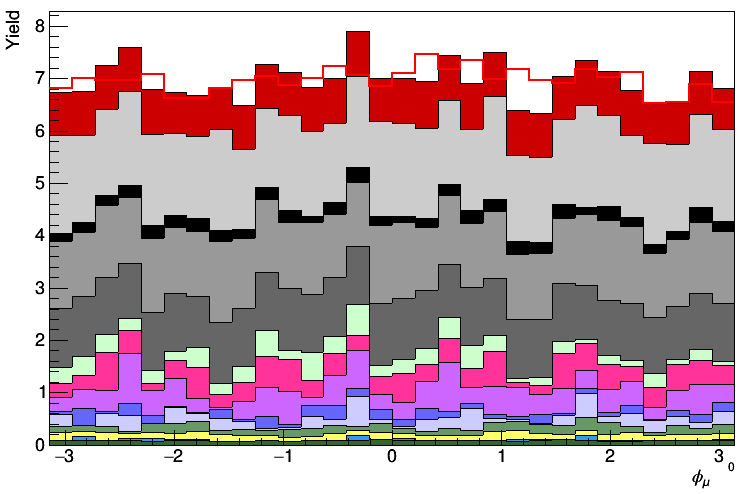
\includegraphics[width=.99\linewidth]{figs/featuresRNN/mu_phi_0}
\end{subfigure}
\begin{subfigure}{.5\textwidth}
  \centering
  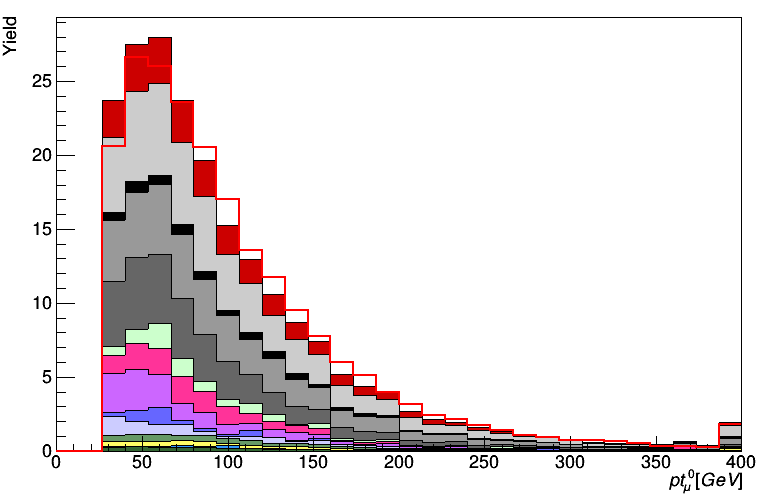
\includegraphics[width=.99\linewidth]{figs/featuresRNN/mu_pt_0}
\end{subfigure}
\caption{Input features of the Recurrent Neural Network.}
\end{figure}




\section*{Additional Plots}
\label{ap:addRNN}

\begin{figure}[H]
\begin{subfigure}{.5\textwidth}
  \centering
  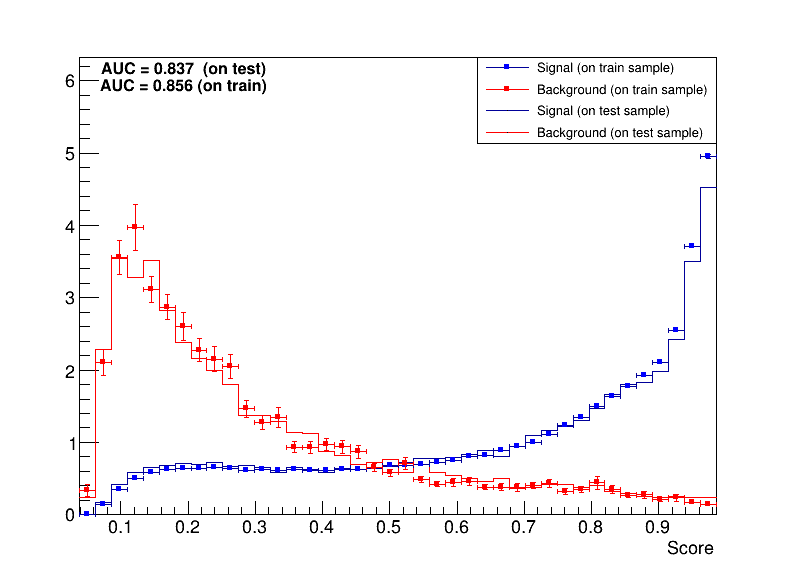
\includegraphics[width=.99\linewidth]{figs/RNN/ScoreLSTMEven}
  \caption{}
  \label{fig:ScoreRNNEven}
\end{subfigure}%
\begin{subfigure}{.5\textwidth}
  \centering
  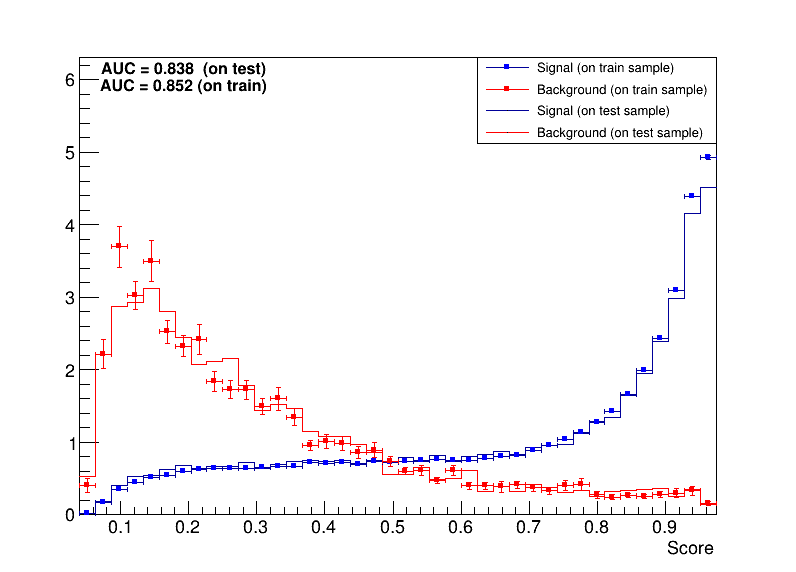
\includegraphics[width=.99\linewidth]{figs/RNN/ScoreLSTMOdd}
  \caption{}
  \label{fig:ScoreRNNOdd}
\end{subfigure}
\caption{Observed Neural Network scores for the RNNs trained with the background dataset containing even event numbers (a) and on the background dataset constraining odd event numbers (b).}
\label{fig:ScoresRNN}
\end{figure}

\begin{figure}[H]
\centering
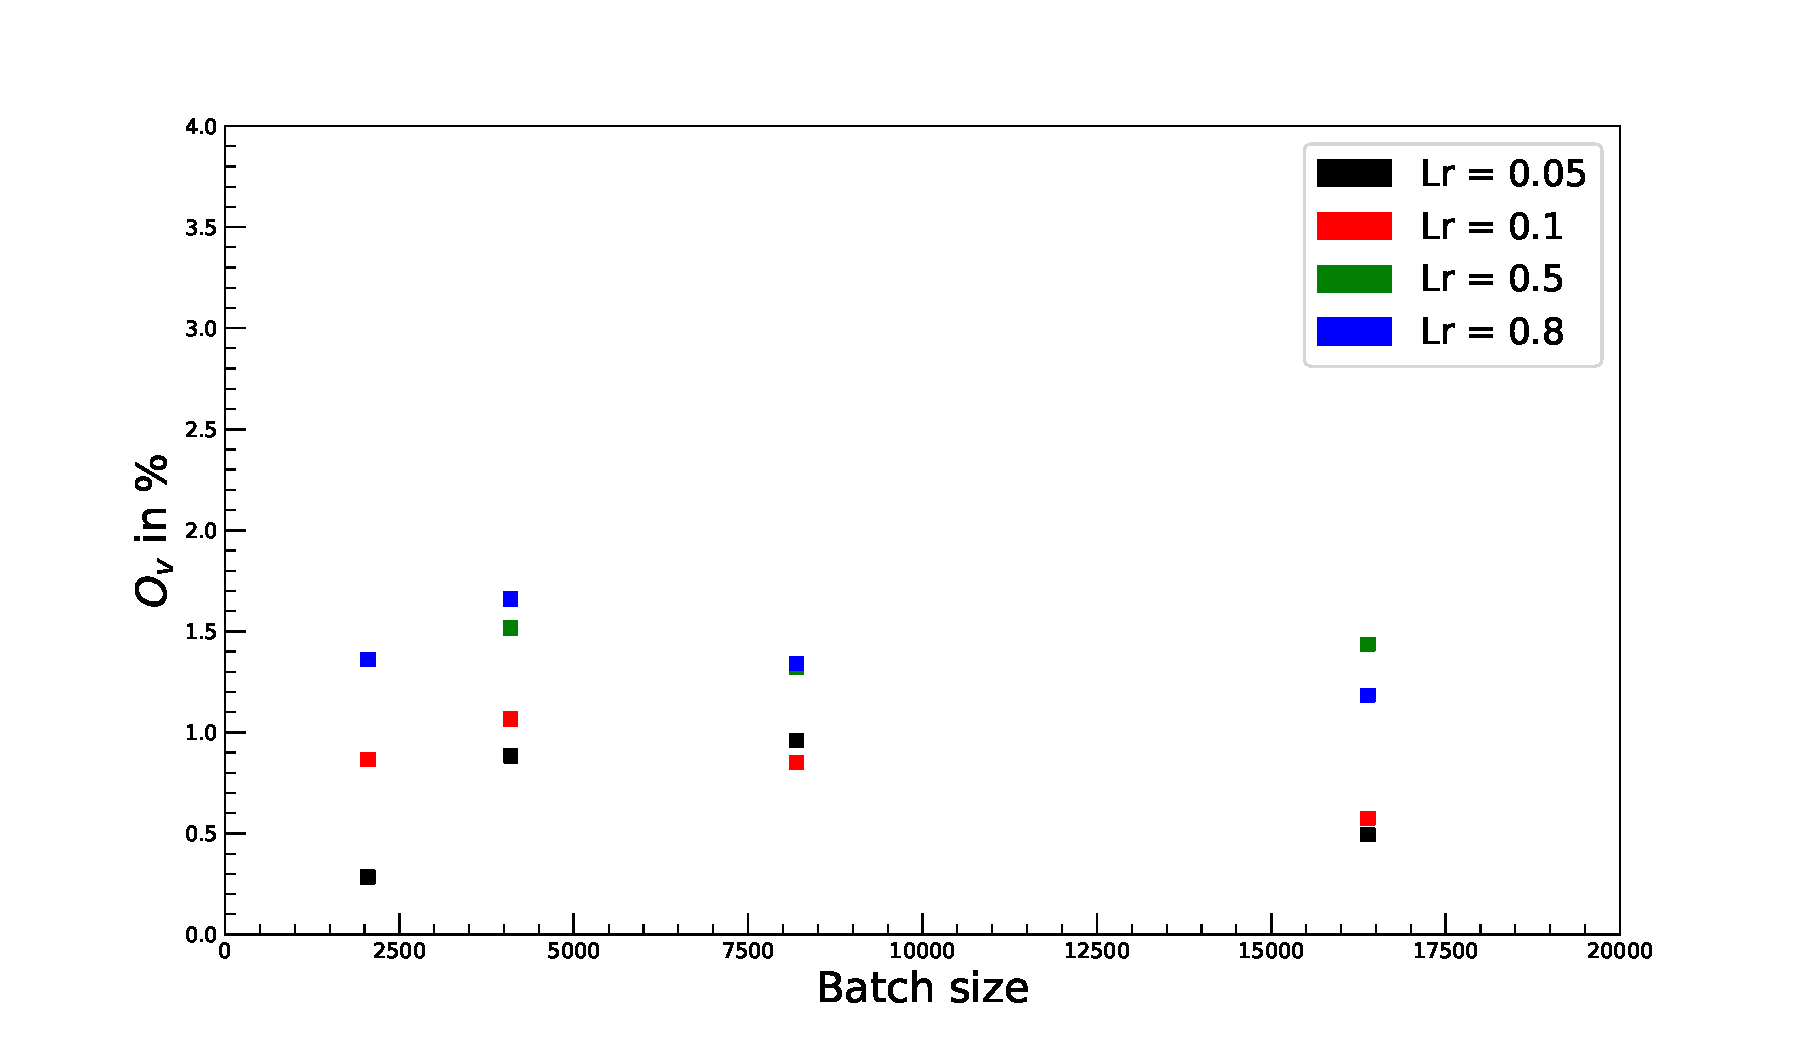
\includegraphics[width=\linewidth]{figs/RNN/BatchOV}
\caption{The overtraining as a function of the batch size and the learning rate.}
\label{fig:Batch1}
\end{figure}

\begin{figure}[H]
\centering
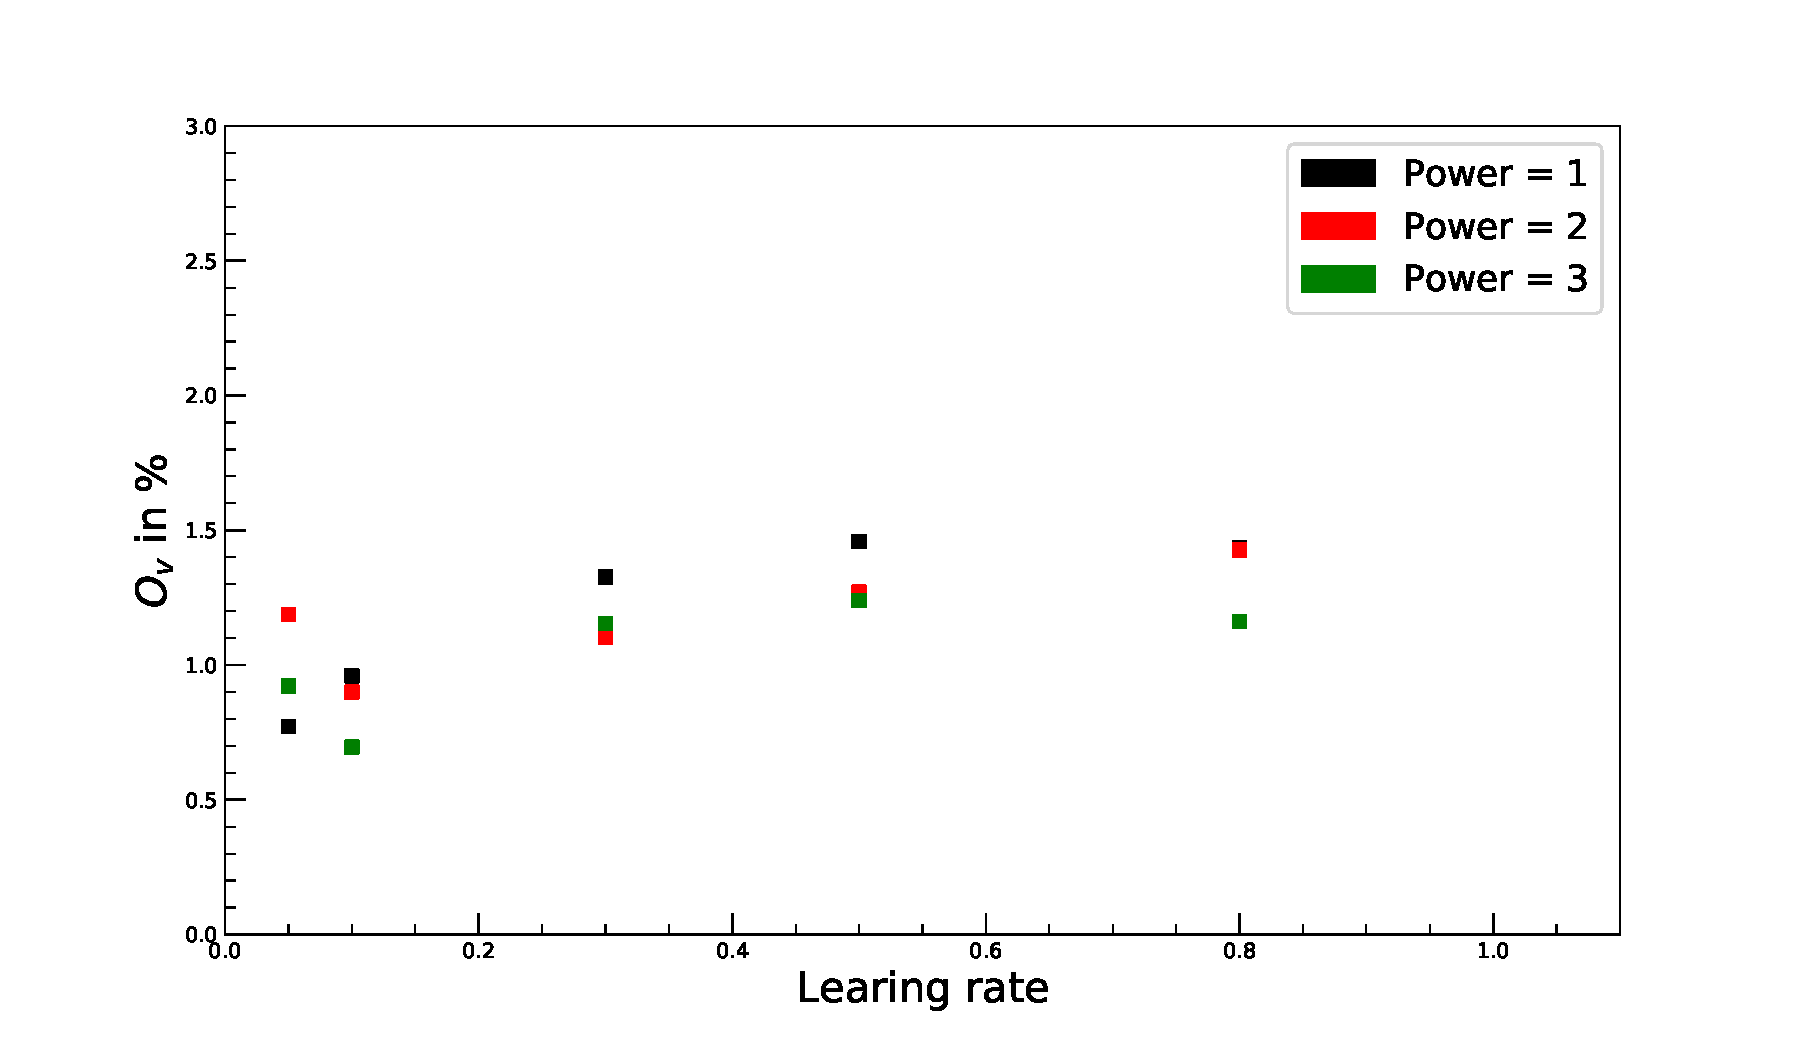
\includegraphics[width=\linewidth]{figs/RNN/LrOv_Fixed}
\caption{The overtraining as a function of the learning rate and the power of the decaying polynomial.}
\label{fig:Batch2}
\end{figure}

\begin{figure}[H]
\centering
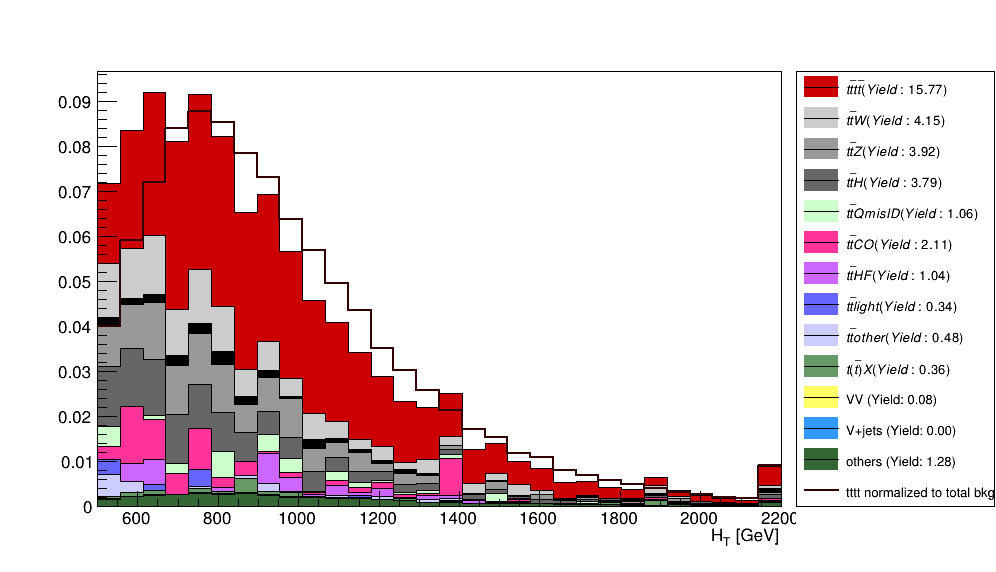
\includegraphics[width=\linewidth]{figs/RNN/HT_all_Odd}
\caption{The $H_{\text{T}}$ distribution after applying a cut (optimized on the signal efficiency) to the RNN score obtained for the training on the background dataset containing odd event numbers. The last bin additionally contains all events with $H_{\text{T}} > 2200$.}
\label{fig:RNNOdd}
\end{figure}
